\section{Dataset}
    \paragraph{}The dataset at the core of this thesis, as previously introduced (see \ref{seq:background:dataset}), consists of heap dump raw files related to different OpenSSH use cases and versions. Each heap dump file is paired with a JSON annotation file created by the dataset's creators. These JSON files provide extra information about the heap dump, especially regarding encryption keys. In this section, we will explain our exploration of the dataset, aiming to better comprehend its content and nuances.

    \subsection{Origin}
        \paragraph{}The dataset is derived from heap dumps that capture various OpenSSH usage scenarios. These scenarios encompass four distinct SSH interactions: a straightforward client connection to the server followed by an immediate exit, port-forwarding, secure copying, and SSH shared connection. The heap dumps span different OpenSSH versions and a range of key sizes, from 16 to 64 bytes. These dumps were generated using the SmartKex tool \cite{fellicious_smartkex_2022}. The data collection was conducted on a mini PC equipped with an AMD Ryzen 5500U processor, 16GB of RAM, and a 1TB NVMe SSD, running Debian 11 as its operating system.

    \subsection{Estimating the dataset balancing for key prediction}
        \paragraph{}In this part, our primary objective was to assess the balance of the dataset for key prediction and identify the challenges associated with it.

        \paragraph{}To begin, we aimed to gain an understanding of the dataset's scale. We utilized a code snippet \ref{methods:code:count_all_dataset_files} to count all the files within the dataset, revealing a total of 208,745 files. However, it was imperative to recognize that JSON files, which served as annotation files, were not to be considered part of the raw bytes for embedding. Consequently, these JSON files were excluded from our count to provide a more accurate representation of the dataset's size.

        \begin{lstlisting}[caption={Count all dataset files}, label=methods:code:count_all_dataset_files, language=bash]
        find . -type f | wc -l
        \end{lstlisting}

        \paragraph{}Following this, we employed another code snippet \ref{methods:code:count_raw_files} to specifically count the heap dump raw files, excluding JSON files. This count indicated a total of 103,595 heap dump raw files, which constituted the primary focus of our analysis.

        \begin{lstlisting}[caption={Count heap dump raw dataset files}, label=methods:code:count_raw_files, language=bash]
        find . -type f -name "*.raw" | wc -l
        \end{lstlisting}

        \paragraph*{}To gain further insights into the dataset, we determined its size while excluding annotation files \ref{methods:code:get_dataset_size}. The calculated dataset size amounted to 18,067,001,344 bytes.

        \begin{lstlisting}[caption={Get the size of the dataset}, label=methods:code:get_dataset_size, language=bash]
        find . -type f -name "*.raw" -exec du -b {} + | awk '{s+=$1} END {print s}'
        \end{lstlisting}

        \paragraph{}Considering the nature of the dataset, which featured a maximum of six keys per file, each with a maximum size of 64 bytes, we conducted a rough estimate. We determined that the maximum number of bytes relevant for searching across the dataset was $6 * 64 * 103595 = 39 780 480$ . This calculation accounted for approximately 0.22\% of the dataset's total size.

        \paragraph{}Lastly, it is crucial to acknowledge that the dataset exhibited a significant imbalance and is very large. To address this challenge effectively, strategies were implemented to ensure robust, unbiased analyses, and scalability.
    \subsection*{Annotations}
        \paragraph{}The annotations files are essential to understand the data and how best to utilize them for the study. Each heap dump corresponds to one specific JSON file. To view the contents of these JSON files in a more organized manner, one can reference the method provided at \ref{methods:code:pretty_print_json}. For a clearer understanding, an extract of the JSON annotation from the file located at \path{./Training/client/V_7_8_P1/16/13116-1644920217.json} is available at \ref{methods:code:annotation_extract}.

        \begin{lstlisting}[caption={pretty print JSON}, label=methods:code:pretty_print_json, language=bash]
            python3 -m json.tool file.json
        \end{lstlisting}

        \noindent
        \begin{minipage}{\linewidth}
        \begin{lstlisting}[language=json, caption={An extract of the JSON annotations}, label=methods:code:annotation_extract]
        {
            /* file ./Training/client/V_7_8_P1/16/13116-1644920217.json*/
            "SSH_STRUCT_ADDR": "5619dd7e5570",
            "SESSION_STATE_ADDR": "5619dd7e5df0",
            "KEY_A_ADDR": "5619dd807f40",
            "KEY_A_LEN": "12",
            "KEY_A_REAL_LEN": "12",
            "KEY_A": "34fbe182e76c49a617a93e2e",
            /*...*/
            "KEY_E_ADDR": "5619dd808000",
            "KEY_E_LEN": "0",
            "KEY_E_REAL_LEN": "0",
            "KEY_E": "",
            "KEY_F_ADDR": "5619dd807fd0",
            "KEY_F_LEN": "0",
            "KEY_F_REAL_LEN": "0",
            "KEY_F": "",
            "HEAP_START": "5619dd7e3000"
        }
        \end{lstlisting}
        \end{minipage}

        \paragraph{}Within these annotation files, several critical pieces of information are present. The ``SSH\_STRUCT\_ADDR'' and ``SESSION\_STATE\_ADDR'' denote the addresses of vital openSSH \glspl{structure}. These addresses are pivotal in gauging the embedding coherence across different openSSH uses and key sizes. If the embeddings of these \glspl{structure} display similarity across various key sizes and openSSH usages, it signifies the embedding's coherence.

        \paragraph{}Other significant annotations such as ``KEY\_A\_ADDR'', ``KEY\_A\_LEN'', ``KEY\_A\_REAL\_LEN'', and ``KEY\_A'' detail the address, length, and value of the key A. In general, six of these annotations can be found for each heap dump. Notably, the ``HEAP\_START'' annotation, along with the length of the heap dump, is of paramount importance. This annotation signifies the starting address of the heap dump. This information not only aids in pinpointing addresses in the heap dump for \glspl{structure} and \glspl{pointer}, but also refines the heuristic used in detecting \glspl{pointer} \ref{seq:background:pointers_and_structures}. By leveraging the ``HEAP\_START'' information, one can verify if a \gls{pointer} is pointing within the heap dump boundaries. As a practical illustration, deducing the address of key A within the heap dump can be achieved by subtracting ``HEAP\_START'' from ``KEY\_A\_ADDR''.

        \paragraph{}However, it's noteworthy that some of these annotation files may be corrupted. Therefore, it's imperative to verify the integrity of each file before its use. In instances where keys are corrupted, such as "KEY\_E" and "KEY\_F" having no recorded values in the extract found at \ref{methods:code:annotation_extract}, it's advised either to remove the corrupted keys or discard the entire file if the data cannot be salvaged. Armed with this understanding, the next logical step would be to leverage this dataset to formulate embeddings and subsequently evaluate their performance.

    \subsection{Malloc header usage and structures detection}
        \paragraph{}As discussed in \ref{seq:background:pointers_and_structures}, subsequent to an initial 8-byte block of zeros, we anticipate the allocation of the first data structure at the heap's commencement. As illustrated in \ref{fig:methods:malloc_header_detection_heap_start}, this data structure spans a size of $ 5102000000000000_{16LE} $ (in little-endian hexadecimal notation) or $ 593_{10} $ bytes. The presence of an odd number arises from the \acrshort{lsb} being set to 1, signifying that the block is allocated (as a flag). Consequently, the actual size of the structure is $ 593_{10} - 1_{10} = 592_{10} $ bytes, which aligns with an 8-byte boundary.

        \begin{figure}[H]
            \centering
            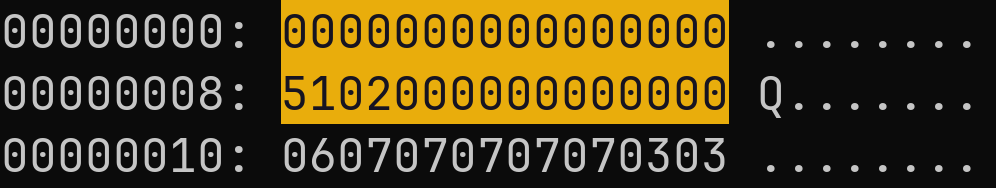
\includegraphics[width=16cm]{background/structure_examples_1010-1644391327-heap_potential_malloc_header_highlight_heap_start.png}
            \caption{Attempt at malloc header detection in \textit{Training/basic/V\_7\_8\_P1/16/5070-1643978841-heap.raw}, at heap start.}
            \label{fig:methods:malloc_header_detection_heap_start}
        \end{figure}

        \paragraph{}Given the allocator's sequential chunk allocation approach, the subsequent chunk's anticipated allocation address is calculated as $ 5102000000000000_{16LE} + 592_{10} + 8_{10} $. The additional 8 accounts for the malloc header block, resulting in an address of $ 5882193a34560000_{16LE} $.
    
        \paragraph{}In vim, since the address start at 0, we have to look at $ 592_{10} + 8_{10} = 258_{16} $. Let's have a look there \ref{fig:methods:malloc_header_detection_0x250}:

        \begin{figure}[H]
            \centering
            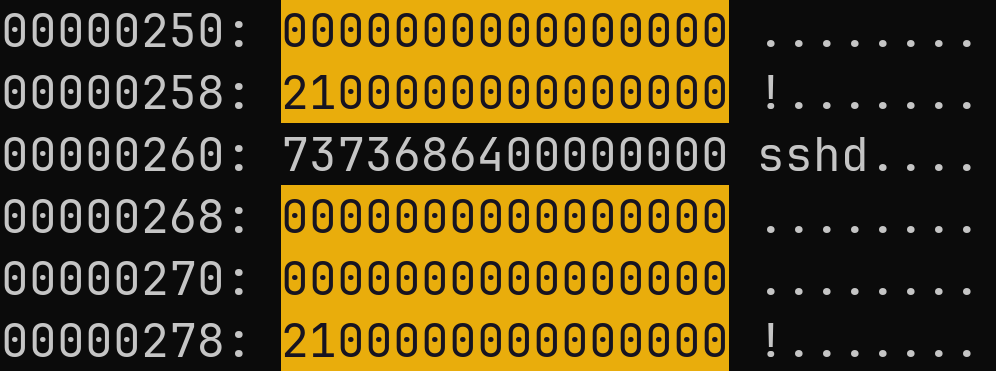
\includegraphics[width=16cm]{background/structure_examples_1010-1644391327-heap_potential_malloc_header_highlight_0x250.png}
            \caption{Attempt at malloc header detection in \textit{Training/basic/V\_7\_8\_P1/16/5070-1643978841-heap.raw}, at index $ 592_{10} = 250_{16} $.}
            \label{fig:methods:malloc_header_detection_0x250}
        \end{figure}

        \paragraph{}At this point, we observe a zero block, succeeded by a potential malloc header at address $ 258_{16} $. By replicating this process, we can devise an algorithm to identify malloc headers, and consequently, the structures within the heap dump file.

        \begin{algorithm}[H]
            \caption{Malloc Header Detection Algorithm}
            \begin{algorithmic}[1]
            \Procedure{MallocHeaderDetection}{$\text{heapDumpFile}$}
                \State $\text{position} \gets 0$
                \While{$\text{position} < \text{FileSize}(\text{heapDumpFile})$}
                    \State $\text{block} \gets \text{Read8Bytes}(\text{heapDumpFile, position})$
                    \If{$\text{block} \neq 0$}
                        \State $\text{size} \gets \text{ConvertToSize}(\text{block}) - 1$ \Comment{$-1$ due to the flag}
                        \State \textbf{Assert} $ \text{size} \mod 8 = 0$ \Comment{Check if the size is 8-bytes aligned}
                        \State $\text{position} \gets \text{position} + 8 + \text{size}$ \Comment{Leap over data structure. + 8 for the header.}
                    \Else
                        \State $\text{position} \gets \text{position} + 8$
                    \EndIf
                \EndWhile
            \EndProcedure
            \end{algorithmic}
        \end{algorithm}

        \paragraph{}The underlying concept of the malloc header detection algorithm is straightforward. Beginning at the start of the heap dump file, we search for the initial non-zero block. Subsequently, we infer that the following block represents a malloc header. This block is converted into a size, allowing us to skip over both the data structure and its header. This procedure continues iteratively until the file's conclusion.
